\documentclass{article}
\usepackage{subfigure,graphicx}
\usepackage{amssymb}

\title{Clustering of Time Series using Wavelet Transformations as a Feature Extraction Mechanism}
\author{\textsf{Kathy Norman, Ssurey Moon, Felix Huang, Josu\'e Kuri}\\UCSC Extension. 30164:(003) Machine Learning and Data Mining}

\begin{document}
\maketitle

\section{Introduction}
A time series is a sequence of data points indexed by time at regular intervals. This model is used to represent a wide range of metrics such as the daily closing price of stocks, temperature, precipitation, population, etc. In the context of machine learning and data mining, clustering of a large set of time series is an exploratory technique aimed at identifying and understanding underlying patterns.

Considering every point of a time series as a dimension results in a high dimensional space which clustering algorithms cannot handle easily. These algorithms depend on a distance measure as a basis to maximize cohesion and separation. In a high dimensional space, the contrast between the nearest and the farthest neighbor becomes smaller making it difficult for clustering algorithms to find meaninful groups \cite{BGRS99}.

Data dimensionality reduction is an approach to map a high dimensional space into a lower dimensional space such that the main characteristics of the data points in the original space are preserved and clustering on the lower dimensionality space results in meaningful groups. The two types of dimensionality reduction are feature selection and feature extraction. The former consists in selecting a subset of features from the original features. Feature extraction, on the other hand, generates a new set of features through a mapping function.

Feature extraction techniques commonly used include Singular Value Decomposition (SVD), Discrete Fourier Transform (DFT) and Discrete Wavelet Transform (DWT). Of these techniques, SDV is the most effective at reconstructing time series with minimal error. However, its time complexity $O(mn^2)$, where $m$ is the number of time series and $n$ is the lenght of each time series, makes this a computally-intensive approach \cite{ZHZL06}. A Fast Fourier Transform (FFT) algorithm can compute DFT coefficients in $O(mn \log n)$ and DWT, using a spacial type of wavelet called {\em Haar wavelet} can achieve $O(mn)$ \cite{ZHZL06}.

In this project we use a feature extraction approach based on DWT using the Haar wavelet as the basis for the transformation. We create a generic framework for clustering of time series using this approach and apply the framework to three types of time series: daily closing stock prices, daily values of exchange rates, and earthquake activity over time for various geographic regions. We use a silhouette coefficient as the criterion to evaluate the quality of the clusterings generated by the framework.


\section{Wavelet transformation}

Wavelet transformation is a time-frequency domain transformation technique for hierarchical decomposition of signals \cite{C92,D92}. The decomposition creates an approximation of the original signal that preseves the trend of the signal, as well as additional data sets that provide increasing levels of detail to reconstruct the original signal. This original signal can be reconstructed without loss of information by applying an inverse wavelet transform to the combination of the approximation signal and all the detail data sets.

Early work on wavelets originated with Morlet in the 1980s as a new tool for seismic signal analysis \cite{MAFG82}. Further work by Morlet, Grossman, Meyer, Mallat and Daubechies \cite{CGT89,D88} broght the concept to the mainstream mathematics community with applications in signal processing, statistics and other areas. There is at present a vast body of literature about the foundations and applications of wavelets. The interested reader is referred to \cite{BGG98} and similar works for a comprehensive presentation of the field.


\section{Wavelet-based feature extraction}

Consider a time series $\overrightarrow{X} \in \mathbb{R}^n$ as an ordered sequence of $n \in 2^J, J \in \mathbb{N}$ numbers. After decomposing $\overrightarrow{X}$ at a resolution $r \in \{2,4,6,8,10, ...\}$, the coefficients associated to the $r$ level can be represented as a sequence $\{A_r,D_r,D_{r-1},...,D_2,D_1\}$. The first element $A_r$ is the approximation coefficients array, and the subsequent elements $D_r,D_{r-1},...,D_2,D_1$ are the details coefficients arrays. In this project we use the vector $\widehat{X} = \{A_r,D_r\}$ at specific levels $r \in \{2,4,6,8,10\}$ as feature vectors for the clustering of a set of time series. The cardinality $|\widehat{X}|$ decreases as $r$ increases. It results, on one hand, in a reconstruction with less fidelity than the original signal $\overrightarrow{X}$ and, on the other hand, on clusterings of potentially better quality because of the smaller dimensionality of $\widehat{X}$.


\section{Experimental evaluation}

The purpose of the experimental evaluation of the generic framework for clustering of time series is to assess the relative efficiency of the framework on a set of contrasting application domains ranging from financial markets to geological phenomena. Variations in the cardinality $|\widehat{X}|$ of feature vectors, the choosen clustering algorithm, as well as the number of clusters, are considered to assess what combination of algorithm and input parameters is the most appropriate for specific situations.

\subsection{Evaluation criteria}
<<<<<<< HEAD
There is no explicit way to evaluate the quality of these time-series clustering systems, since it is of unsupervised learning. In supervised learning data set contains true classes of all data points, and they are used to calculate SSE(Sum of Square Errors) to evaluate the quality of the implementation. In contrast, evaluation of clustering implementation on unsupervised learning data set need another approach to internally calculate the quality of derived clusters. The most popular method is to get cohesion and separation. Cohesion means how close each node in a cluster $\sum_{i} \sum_{j} (x_{i,j}-m_j)^2$ where $i$ is number of clusters, $x_{i,j}$ is a $j_{th}$ node in the cluster $i$, and $m_{i}$ is the center of the cluster $i$. On the other hand, separation means how far each cluster is from others, $\sum_{k} \sum_{i} (m_{k}-m_{i})^2$. The higher those values are, the better nodes are clustered.
Silhouette coefficient takes both concepts of cohesion and separation:\\
\begin{equation}
s = \begin{cases}
1-a/b  \,\,\,\, \mbox{for $a \le b$}  ,\,\,
b/a-1  \,\,\,\, \mbox{otherwise}
\end{cases}
\end{equation}
where $a$ is the average distance $x_{i}$, a random node in the cluster $i$, and other nodes in the cluster, $b$ is the minimum value the average distances of $x_{i}$ and nodes in another cluster $k$. The closer to one the value is, the better nodes are clustered.
In this project we use Silhouette coefficient to measure the performance of our implementation. There are a few parameters to consider, such as clustering algorithm, level of complexity, in other words, feature extraction level, and a forced number of clusters. Silhouette score plots point which combination of parameters performs better on different type of time-series data sets.


The three main criteria used to evaluate clusters are \cite{TSK05}:

\begin{description}
\item[External.] Measure the extent to which cluster labels match externally supplied labels.
\item[Internal.] Measure the goodness of a clustering without respect to external information.
\item[Relative.] Compare two different clusterings.
\end{description}

We evaluate our clustering framework using an internal criterion known as silhouette coefficient. The coefficient is defined as $S = 1-a/b$, where $a$ is a measure of cohesion -how closely related are objects in a cluster-, and $b$ is a measure of separation -how distinct a cluster is from other clusters-. The value of $S$ is typically in $[0,1]$. A clustering with a silhouette coefficient close to $1$ is deemed better than a clustering with a silhouette coefficient close to $0$.

\subsection{Data description}

\subsubsection{Stock closing prices}
This data set consists of the time series of daily closing prices for one hundred stocks from diverse industries (Internet, telecommunications equipment and service providers, entertainment, media, airlines, etc.) between April 20th 2011 and May 16th 2015. The time series represent 1024 trading days, and are normalized using as basis the closing price of the first day of the interval (April 20th 2011). 

\subsubsection{Historic exchange rates}


\subsubsection{Historic earthquake data}



\subsection{Performance evaluation}

\begin{figure}
\begin{center}
\subfigure[Level 2]{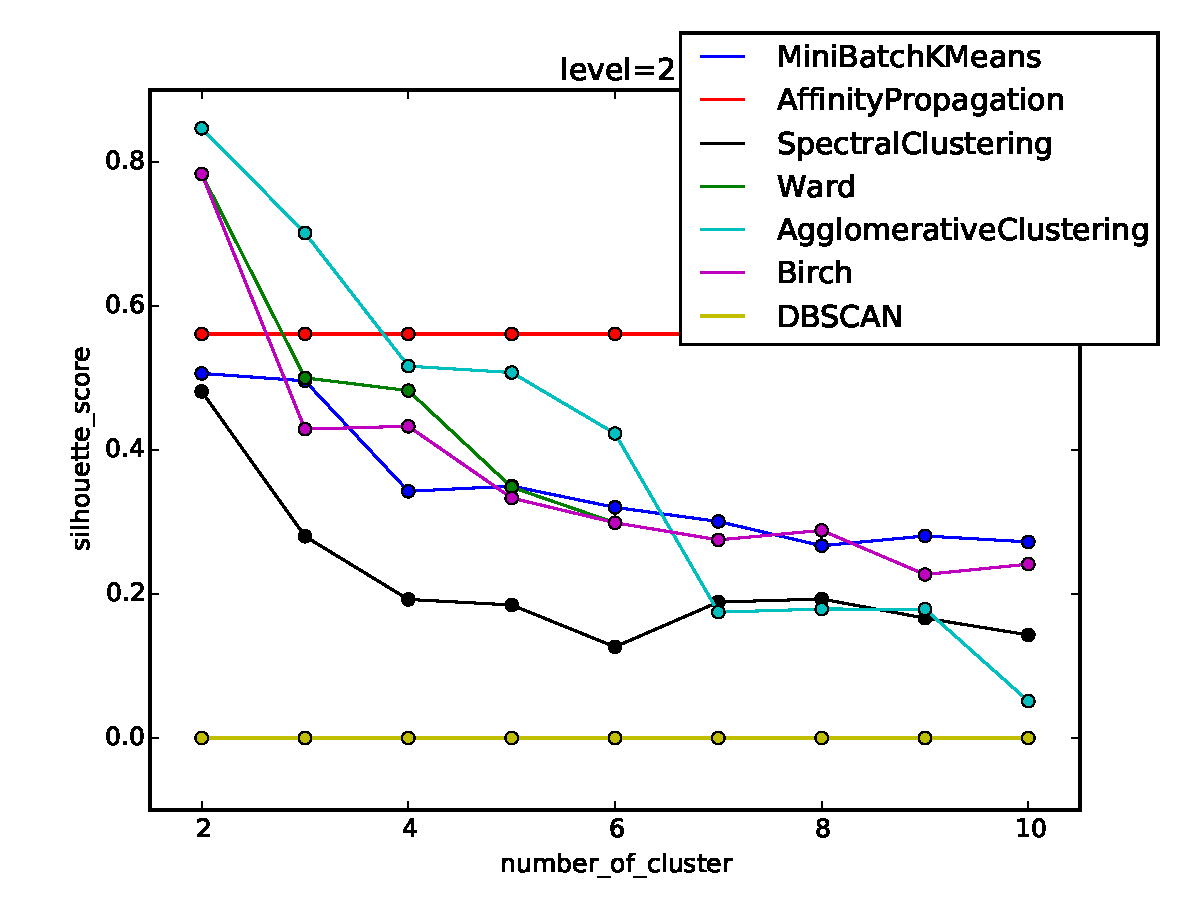
\includegraphics[width=0.49\textwidth]{../task4/silhouette_score_plot_per_number_of_cluster(level=2).pdf}}
\subfigure[Level 4]{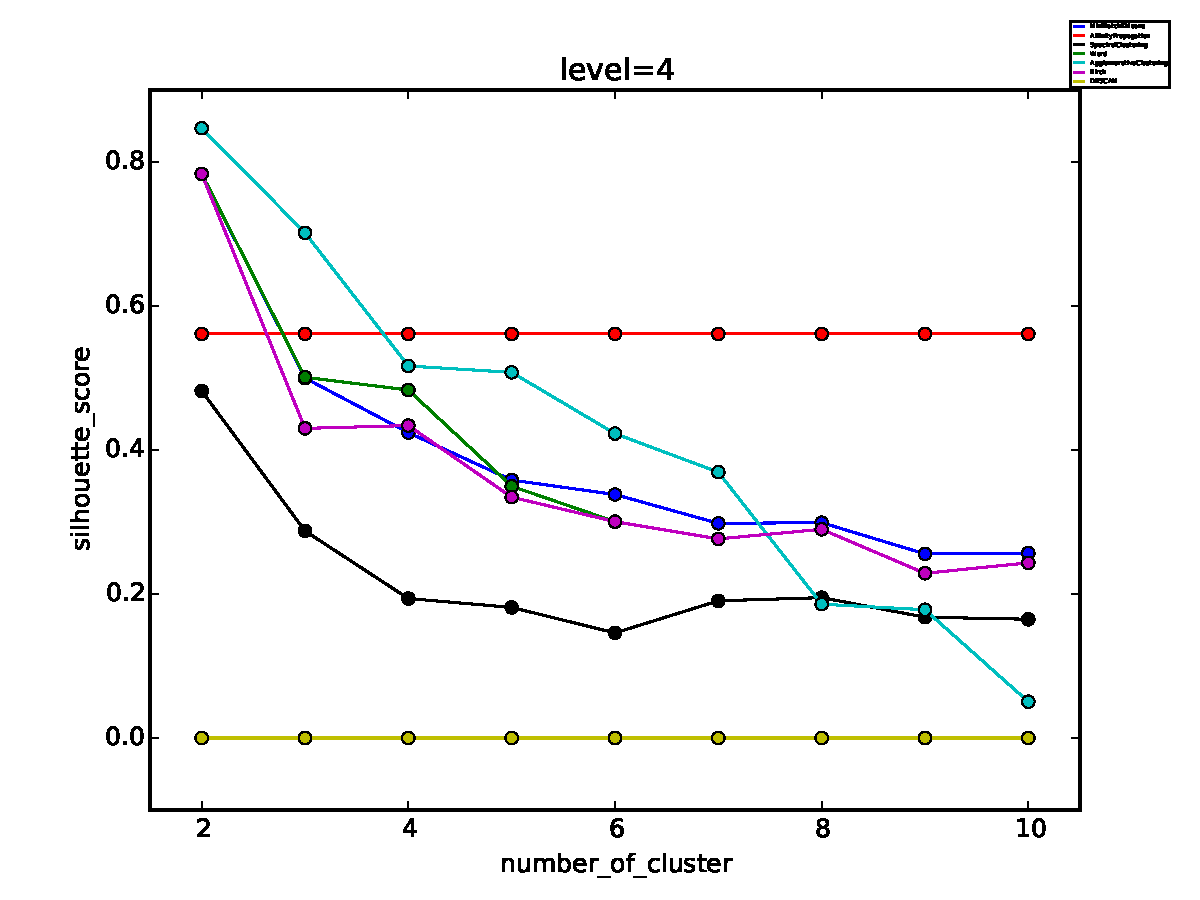
\includegraphics[width=0.49\textwidth]{../task4/silhouette_score_plot_per_number_of_cluster(level=4).pdf}}
\subfigure[Level 6]{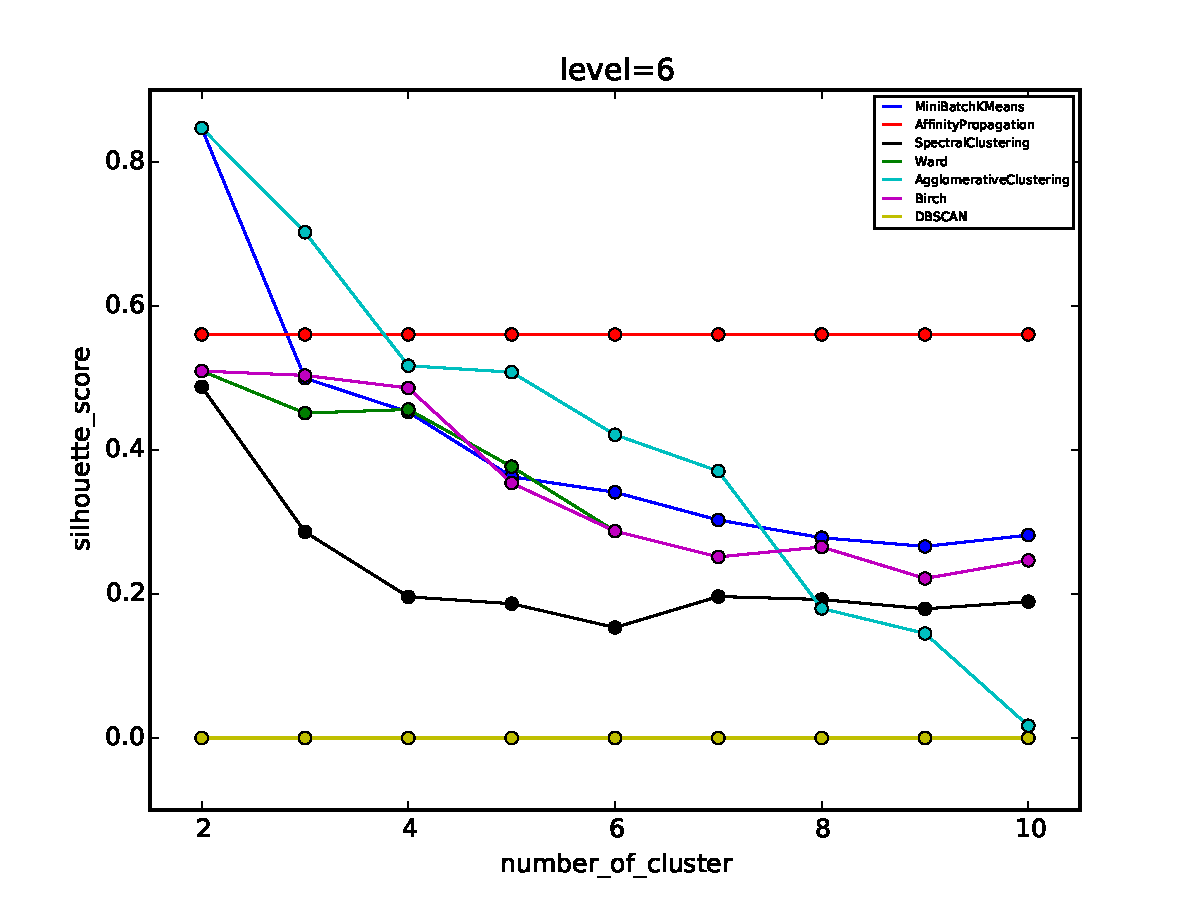
\includegraphics[width=0.49\textwidth]{../task4/silhouette_score_plot_per_number_of_cluster(level=6).pdf}}
\subfigure[Level 8]{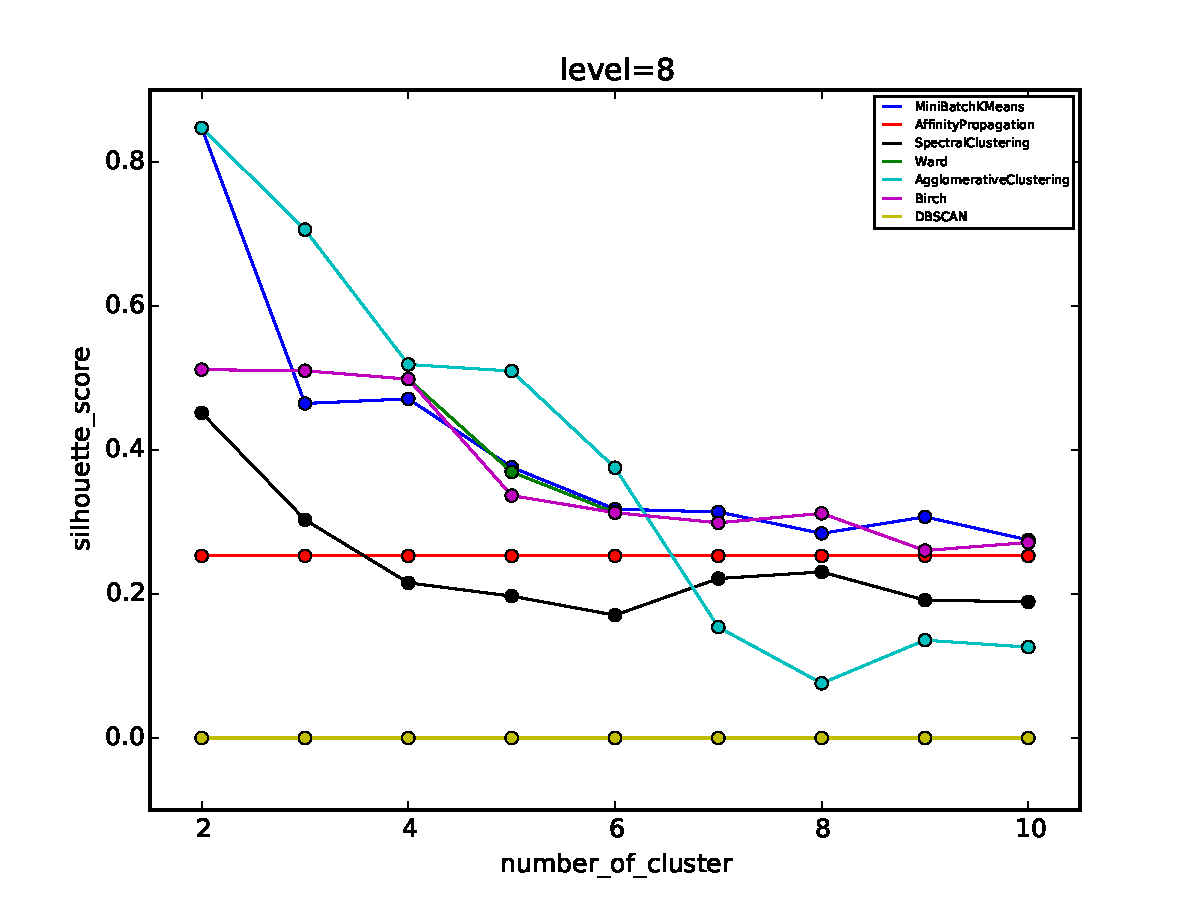
\includegraphics[width=0.49\textwidth]{../task4/silhouette_score_plot_per_number_of_cluster(level=8).pdf}}
\caption{Silhouette score for various clustering levels.} \label{silhouette_levels}
\end{center}
\end{figure}


\begin{figure}
\begin{center}
\subfigure[Two clusters]{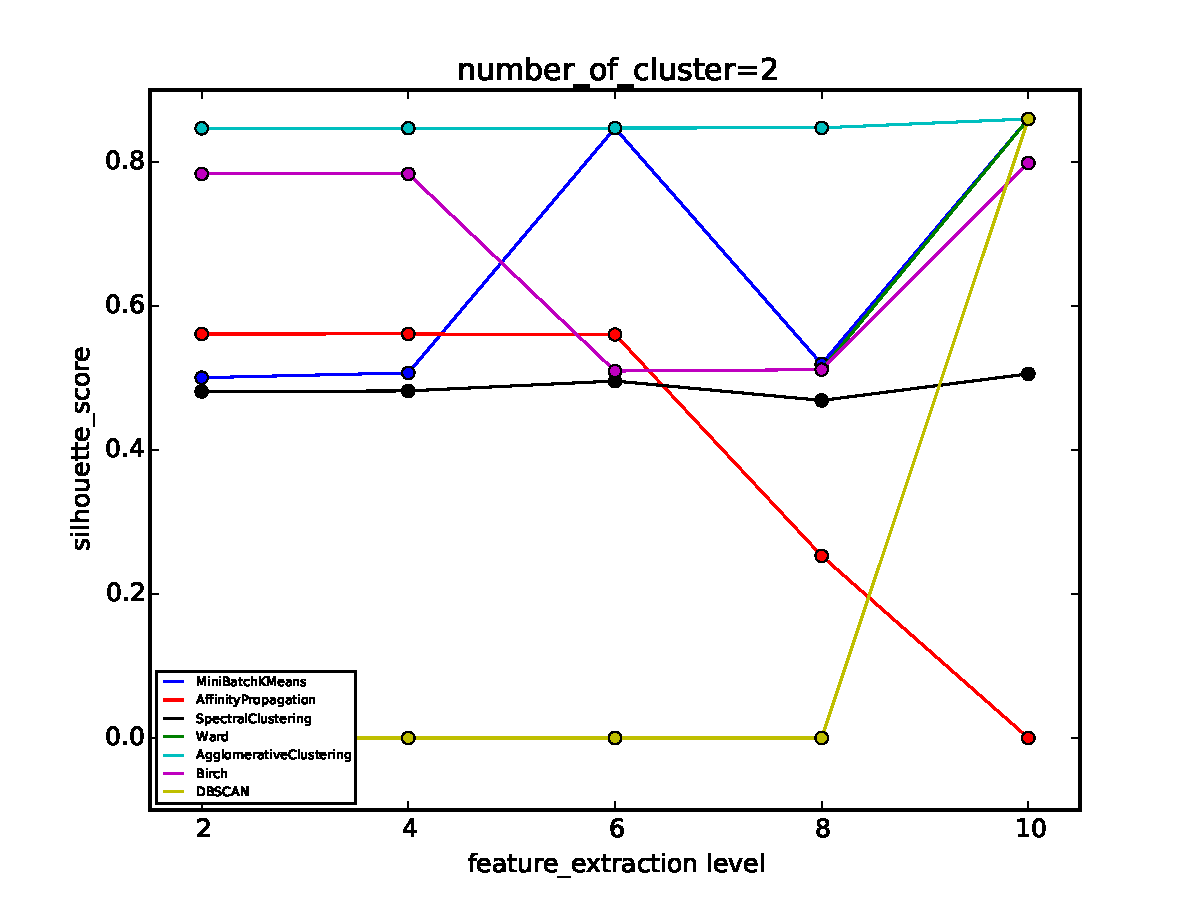
\includegraphics[width=0.49\textwidth]{../task4/silhouette_score_plot_per_level_(clusters=2).pdf}}
\subfigure[Three clusters]{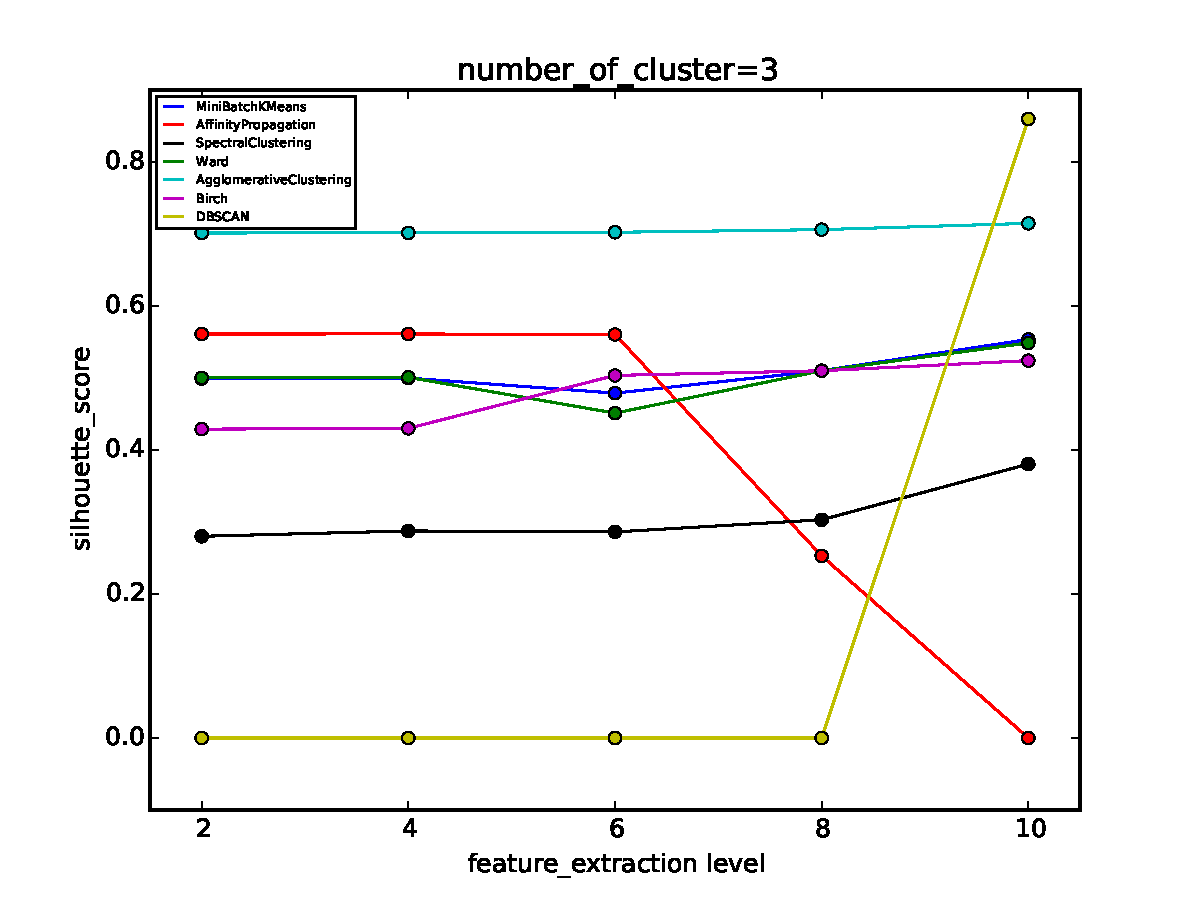
\includegraphics[width=0.49\textwidth]{../task4/silhouette_score_plot_per_level_(clusters=3).pdf}}
\subfigure[Four clusters]{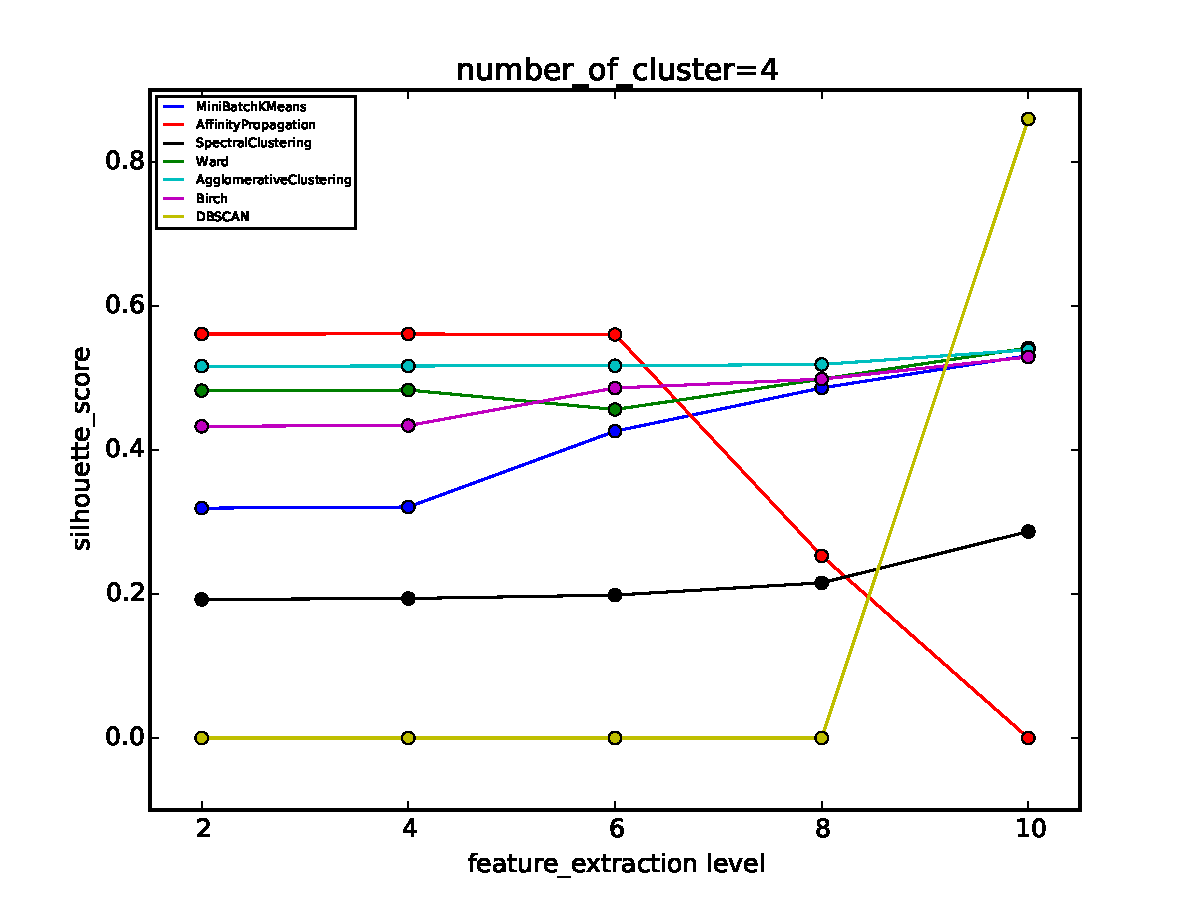
\includegraphics[width=0.49\textwidth]{../task4/silhouette_score_plot_per_level_(clusters=4).pdf}}
\subfigure[Five clusters]{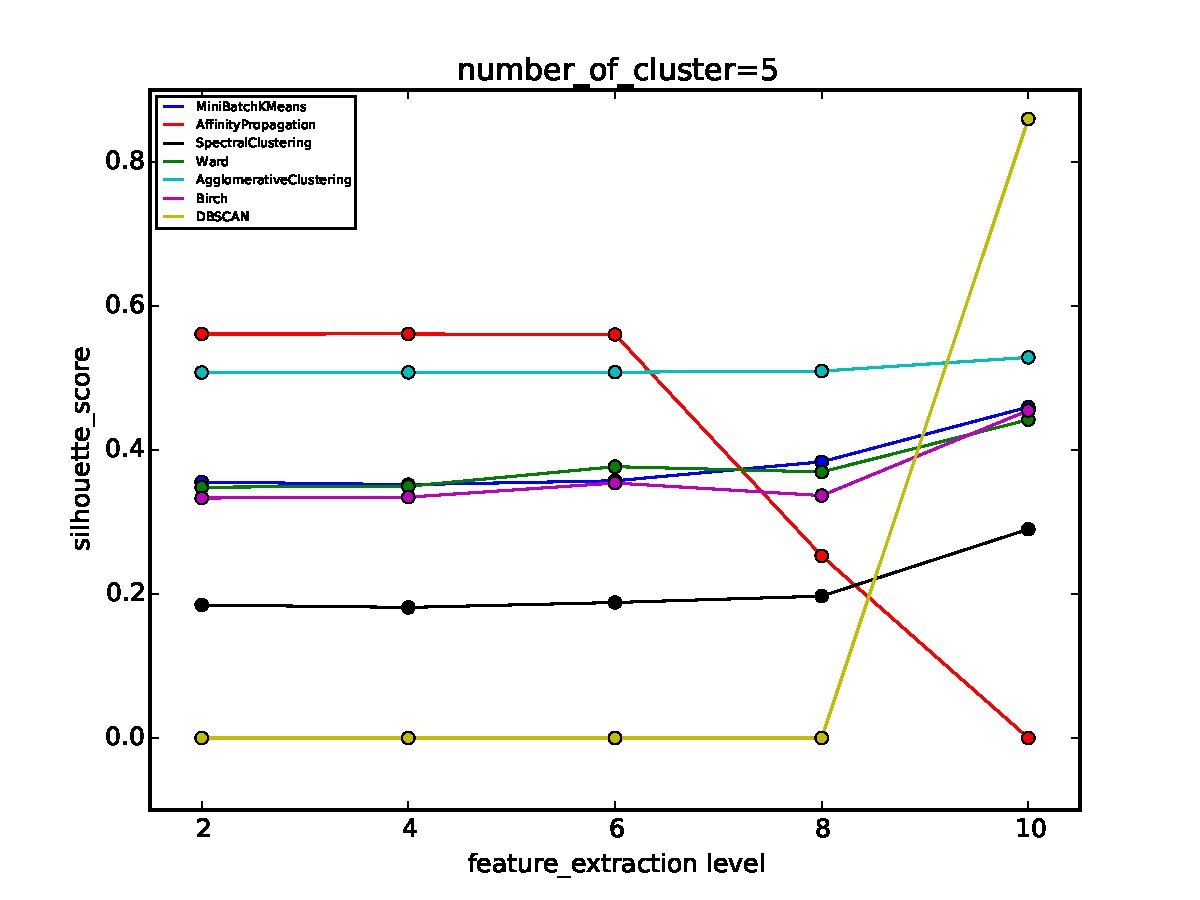
\includegraphics[width=0.49\textwidth]{../task4/silhouette_score_plot_per_level_(clusters=5).pdf}}
\subfigure[Six clusters]{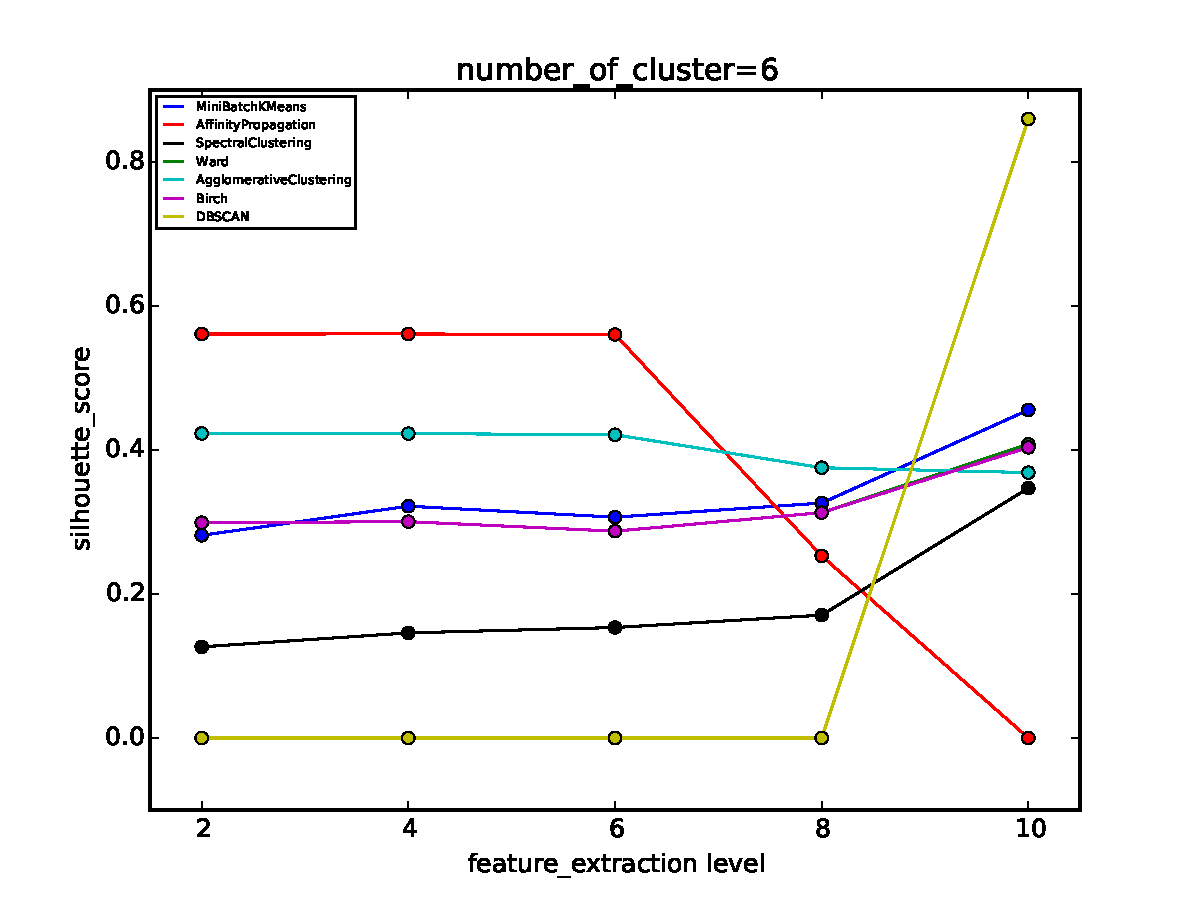
\includegraphics[width=0.49\textwidth]{../task4/silhouette_score_plot_per_level_(clusters=6).pdf}}
\subfigure[Seven clusters]{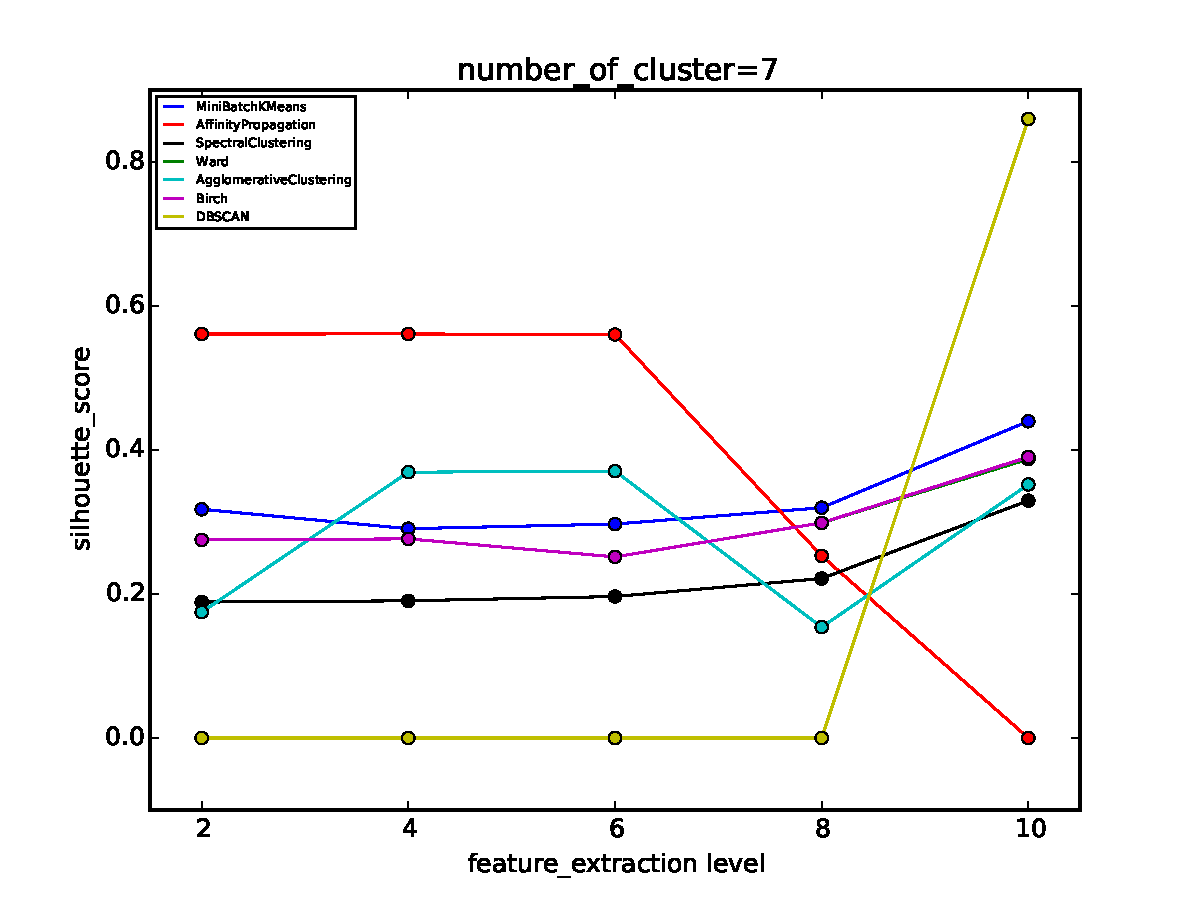
\includegraphics[width=0.49\textwidth]{../task4/silhouette_score_plot_per_level_(clusters=7).pdf}}
\subfigure[Eight clusters]{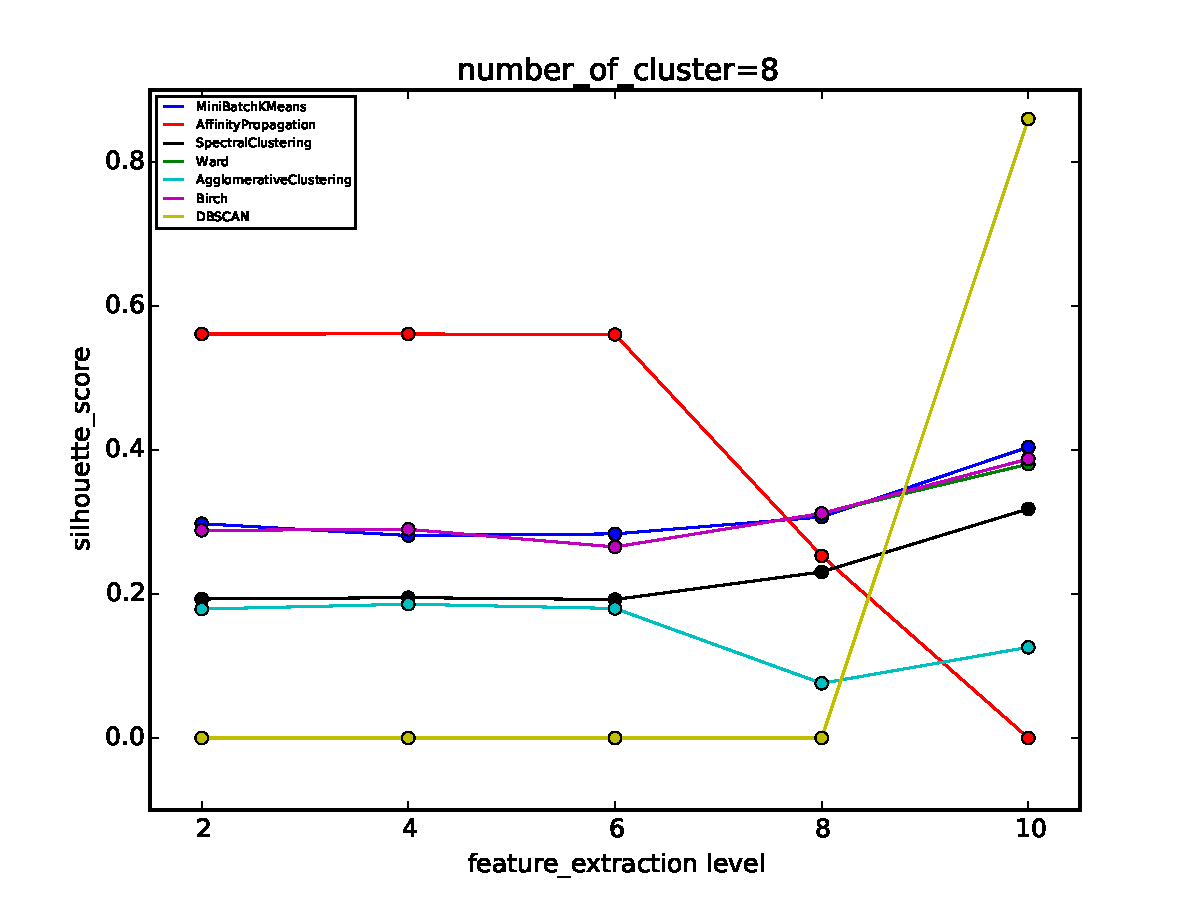
\includegraphics[width=0.49\textwidth]{../task4/silhouette_score_plot_per_level_(clusters=8).pdf}}
\subfigure[Nine clusters]{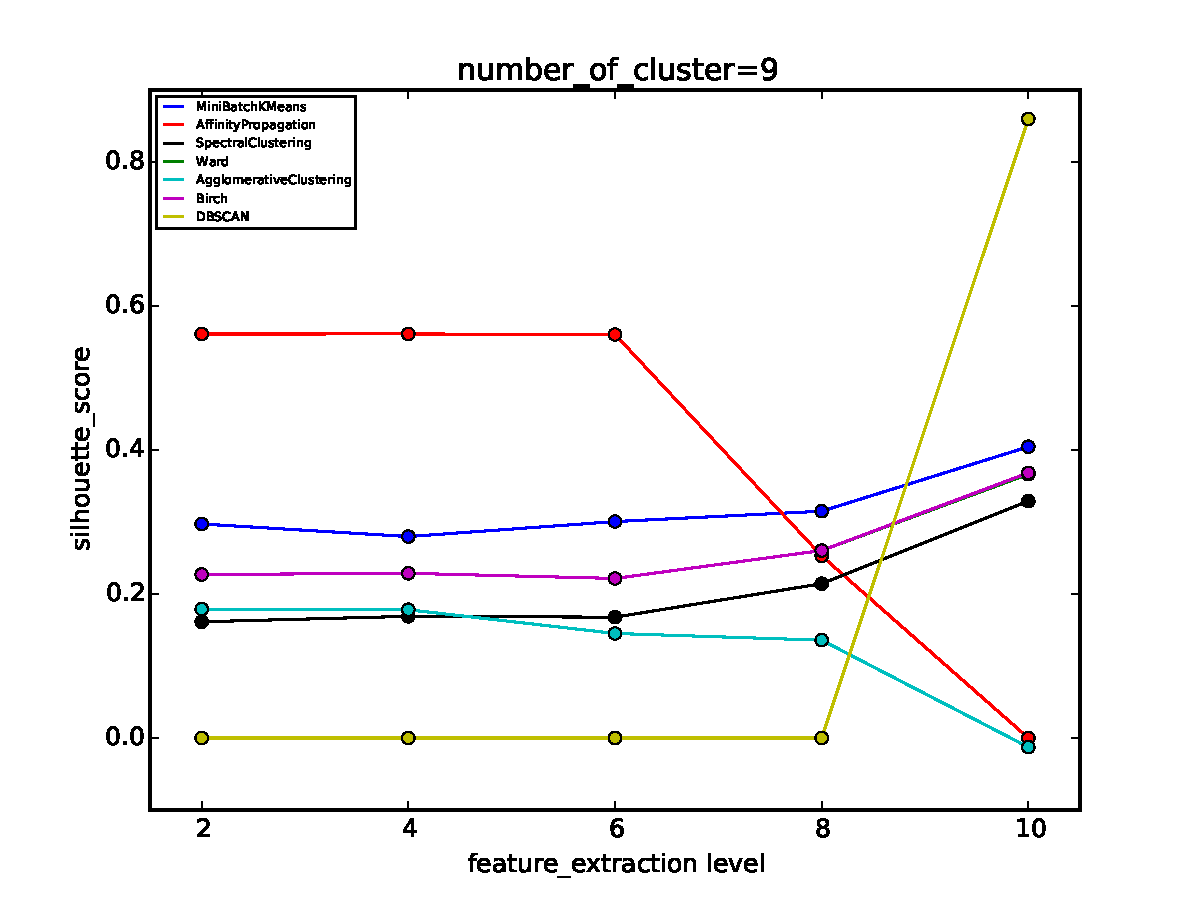
\includegraphics[width=0.49\textwidth]{../task4/silhouette_score_plot_per_level_(clusters=9).pdf}}
\caption{Silhouette score for various clustering levels.} \label{silhouette_levels}
\end{center}
\end{figure}


\section{Conclusions}
Lorem ipsum dolor sit amet, consectetur adipiscing elit, sed do eiusmod tempor incididunt ut labore et dolore magna aliqua. Ut enim ad minim veniam, quis nostrud exercitation ullamco laboris nisi ut aliquip ex ea commodo consequat. Duis aute irure dolor in reprehenderit in voluptate velit esse cillum dolore eu fugiat nulla pariatur. Excepteur sint occaecat cupidatat non proident, sunt in culpa qui officia deserunt mollit anim id est laborum.


  \begin{thebibliography}{1}

\bibitem{BGRS99} K. Beyen, J. Goldstein, R. Ramakrishnan, and U. Shaft. When is nearest neighbor meaningful? In {\em Proceedings of the 7th International Conference on Database Theory}, pp. 217-235, 1999.

\bibitem{ZHZL06} H. Zhang, T. B. Ho, Y. Zhang, M.-S. Lin. Unsupervised Feature Extraction for Time Series Clustering Using Orthogonal Wavelet Transform. In {\em Informatica}, Volume 30, pp. 305-319, 2006.

\bibitem{C92} C. K. Chui. {\em An Introduction to Wavelets.} Academic Press, San Diego, 1992.

\bibitem{D92} I. Daubechies. Ten Lectures on Wavelets. {\em SIAM}, Philadelphia, PA, 1992.

\bibitem{MAFG82} J. Morlet, G. Arens, E. Fourgeau and D. Giard. Wave propagation and sampling theory, Part 1: Complex  signal land scattering in multilayer media. {\em Journal of Geophysics,} 47:203-221, 1982.

\bibitem{CGT89} J. M. Combes, A. Grossman and P. Tchamitchian, editors. {\em Wavelets, Time-Frequency Methods and Phase Space.} Springer-Verlag, Berlin 1989.

\bibitem{D88} I. Daubechies. Orthonormal bases of compactly supported wavelets. {\em Communications on Pure and Applied Mathematics,} 41:909-996, 1988.

\bibitem{BGG98} C. Sidney Burrus, R. A. Gopinath, and H. Guo, {\em Introduction to Wavelets and Wavelet Transforms: A Primer,} Prentice Hall, NJ 1998.

\bibitem{TSK05} P.-N. Tan, M. Steinbach, and V. Kumar. {\em Introduction to Data Mining,} Pearson, First Edition, 2005.

\end{thebibliography}

\end{document}